\chapter{Logische Schnittstellen}\hypertarget{tsfi.ls}{\label{tsfi.ls}}

In diesem Kapitel werden die logischen Schnittstellen des TOE
beschrieben. 

In den Unterabschnitten dieses Kapitel gibt es zu jeder Schnittstelle eine
grafische Darstellung über die Protokolle, die auf der Schnittstelle zum Einsatz
kommen. Dabei sind diejenigen Protokolle, die zu einer TSFI gehören, orange
markiert. Gelb markierte Protokolle gehören nicht zu einer TSFI. Gepunktet
markierte Protokolle sind Schnittstellen für \nontsf{} Anteile des TOE -- also
\secitem{non-TSFI}. Sie werden trotzdem aufgeführt, da sie als
Außenschnittstelle des TOE beschreibungsrelevant sind.

\clearpage

\hrefsection{tsfi.ls.lan}{\tsfisectionname{ls.lan}}

\lslan{} ist eine logische Schnittstelle zu den Clientsystemen, die physisch
über das LAN (\intf{PS.LAN}) erreichbar sind.

Die Schnittstelle umfasst die folgenden Protokolle,
\tableref{tab:ls.lan.protocols-ports} listet diese Protokolle und die dafür
verwendeten Portnummern.  \figureref{fig:tsfi.ls.lan.protocols} stellt die
Protokolle dar, welche die sicherheitsrelevanten Aspekte des TSFI ausmachen
(vgl. die einleitende Bemerkung zu \chapterref{tsfi.ls}).

\begin{description}
\item[Ethernet] für Netzzugang,
\item[IP] für Routing,	
\item[TCP und UDP] für die Transportschicht,
\item[DHCP] für IP-Adressvergabe im LAN (Client),
\item[TLS] für die Absicherung der Kommunikation der anderen logischen
  Schnittstellen im LAN.
\item[HTTP\_Mgmt] für den Zugriff auf die Management-Schnittstelle
\end{description}

\tableref{tab:ls.lan.protocols-ports} listet die Protokolle und verwendeten
Ports detailreicher auf. Abbildung~\vref{fig:tsfi.ls.lan.protocols} zeigt die
Protokolle der Schnittstelle \lslan{} in Relation zueinander und bezogen auf das
TCP/IP Schichtenmodell. Der Protokollstapel ist aus Platzgründen auf zwei
Abbildungen aufgeteilt.

\afterpage{%
  \clearpage% Flush earlier floats (otherwise order might not be correct)
  \begin{landscape}% Landscape page
    \centering % Center table
    {
      \label{tab:ls.lan.protocols-ports}
\begin{longtable}{@{}lcllcclp{6cm}@{}}
  \toprule
  Service & In/Out & Protocol & via & Source port & Dest. port & TSFI & Note \\ \midrule \endhead
  \bottomrule \caption*{Protocols und port numbers for IP/TCP/UDP on \formatintf{LS.LAN}} \endfoot
  \bottomrule \caption{Protocols und port numbers for IP/TCP/UDP on \formatintf{LS.LAN}} \endlastfoot
  Base protocols & -- & IEEE802.3 &  -- & -- & -- &    \tsfilink{ls.lan.ether} \\
  & -- & IPv4 & IEEE802.3 & -- & -- &    \tsfilink{ls.lan.ip} \\
  & -- & TCP &  IPv4 & -- & -- &    \tsfilink{ls.lan.tcp} \\
  & -- & UDP &  IPv4 & -- & -- &    \tsfilink{ls.lan.udp} \\[2ex]
  Administration & In & TLS & TCP & any & 9443 & \tsfilink{ls.lan.tls} & \\ 
  & In & HTTP & TLS & any & 9443 &  \tsfilink{ls.lan.httpmgmt} \\[2ex]
\end{longtable}


%

%!TEX root = "../adv_fsp"
%%% Local Variables:
%%% mode: latex
%%% TeX-engine: luatex
%%% TeX-master: "../adv_fsp"
%%% TeX-parse-self: t
%%% TeX-auto-save: t
%%% End:

    }
  \end{landscape}
  \clearpage% Flush page
}

\begin{figure}[htbp]
  \centering
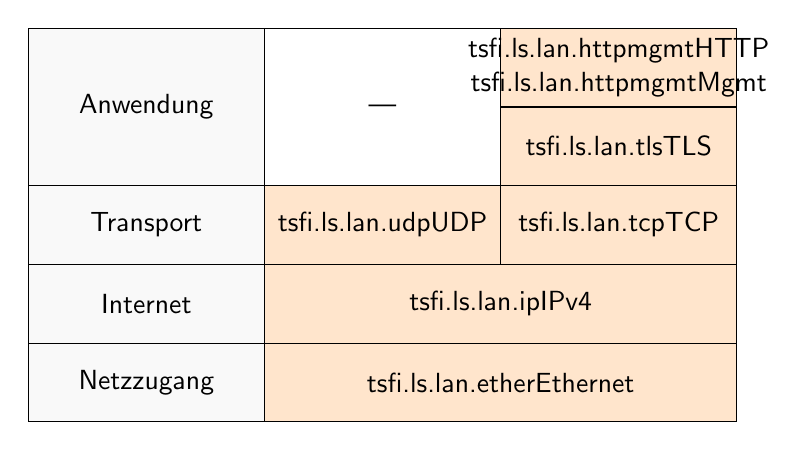
\begin{tikzpicture}
    [c/.style={midway,align=center,font=\sffamily},
      tsfi/.style={fill=orange!20},
      nontsfi/.style={fill=yellow!20},
      none/.style={},
      layer/.style={fill=gray!5}]


  % App Layer für UDP
  \draw[layer] (0,3) rectangle ++(3,2) node[c]{Anwendung};
  \draw[none] (3,3) rectangle ++(3,2) node[c]{---};
  \draw[tsfi] (6,3) rectangle ++(3,1) node[c]{\hyperlink{tsfi.ls.lan.tls}{TLS}};

  \draw[tsfi] (6,4) rectangle ++(3,1) node[c]{\hyperlink{tsfi.ls.lan.httpmgmt}%
    {HTTP}\\\hyperlink{tsfi.ls.lan.httpmgmt}{Mgmt}};

  % Transport Layer
  \draw[layer] (0,2) rectangle ++(3,1) node[c]{Transport};
  \draw[tsfi] (3,2) rectangle ++(3,1) node[c]{\hyperlink{tsfi.ls.lan.udp}{UDP}};
  \draw[tsfi] (6,2) rectangle ++(3,1) node[c]{\hyperlink{tsfi.ls.lan.tcp}{TCP}};

  % IP Layer
  \draw[layer] (0,1) rectangle ++(3,1) node[c]{Internet};
  \draw[tsfi] (3,1) rectangle ++(6,1) node[c]{\hyperlink{tsfi.ls.lan.ip}{IPv4}};

  % Network Layer
  \draw[layer] (0,0) rectangle ++(3,1) node[c]{Netzzugang};
  \draw[tsfi] (3,0) rectangle ++(6,1) node[c]{\hyperlink{tsfi.ls.lan.ether}{Ethernet}};

\end{tikzpicture}
  \caption{Protokolle auf \formatintf{LS.LAN} für die sicherheitsfunktionalen Anteile}
  \label{fig:tsfi.ls.lan.protocols}
\end{figure}

\clearpage

\hrefsubsection{tsfi.ls.lan.ether}{\tsfisectionname{ls.lan.ether}}

\tsfipurpose{tsfi.ls.lan.ether}

Diese Schnittstelle dient als \emph{Netzzugangsschicht} zum
Ethernet-Netzwerk.

\aufgerufenesf{ls.lan.ether}

\tsfiparameters{tsfi.ls.lan.ether}

Die Schnittstelle implementiert das Ethernet-Protokoll nach
\autocite{IEEE802.3}. 

\hrefsubsection{tsfi.ls.lan.ip}{\tsfisectionname{ls.lan.ip}}

\tsfipurpose{tsfi.ls.lan.ip}

Auf der \emph{Internetschicht} verhält sich der TOE als IP-Router und
unterstützt das Internet-Protokoll in der Version 4. Zusätzlich wird das
ICMP-Protokoll unterstützt, welches Teil von IPv4 ist.  

\aufgerufenesf{ls.lan.ip}

\tsfiparameters{tsfi.ls.lan.ip}

Die Implementierung von IPv4 entspricht den Vorgaben aus \rfc[c]{791},
\rfc[c]{1812} und den Aktualisierungen in \rfc[c]{2644}. ICMP ist in
\rfc[c]{792} spezifiziert. Die Implementierung von IPv4 wird durch den
Linux-Kernel bereitgestellt.

\hrefsubsection{tsfi.ls.lan.tcp}{\tsfisectionname{ls.lan.tcp}}

\tsfipurpose{tsfi.ls.lan.tcp}

Auf der \emph{Transportschicht} unterstützt der TOE das Transmission
Control Protocol (TCP). 

\aufgerufenesf{ls.lan.tcp}

\tsfiparameters{tsfi.ls.lan.tcp}

Die Implementierung von TCP entspricht den Vorgaben aus
\rfc[c]{793}. Die Implementierung von TCP wird durch den Linux-Kernel
bereitgestellt.


\hrefsubsection{tsfi.ls.lan.udp}{\tsfisectionname{ls.lan.udp}}

\tsfipurpose{tsfi.ls.lan.udp}

Der TOE unterstützt auf der \emph{Transportschicht} zusätzlich das
User Datagram Protocol (UDP). 

\aufgerufenesf{ls.lan.udp}

\tsfiparameters{tsfi.ls.lan.udp}

Die Implementierung von UDP entspricht den Vorgaben aus
\rfc[c]{768}. Die Implementierung von UDP wird durch den Linux-Kernel
bereitgestellt.

\hrefsubsection{tsfi.ls.lan.tls}{\tsfisectionname{ls.lan.tls}}

\tsfipurpose{tsfi.ls.lan.tls}

\lslantls{} wird verwendet, um Verbindungen zu anderen Systemen im LAN
abzusichern. TLS stellt Vertraulichkeit und
Integrität der Verbindungen sicher. Eine Übersicht über die TLS
Verbindungen und deren Konfiguration des TOE ist in Tabelle
\tableref{tab:tlsconnections} zu finden. 

\aufgerufenesf{ls.lan.tls}

\tsfiparameters{tsfi.ls.lan.tls}

Die Implementierung von TLS im TOE setzt \autocite{rfc5246} um. Die Beschreibung
der TLS-Implementierung sowie allen TLS-Verbindungen des TOE gemeinsamen
Parameter und TOE-spezifische Anpassungen der TLS-Implementierung sind in
Kapitel \ref{sf.tls} dokumentiert.

\hrefsubsection{tsfi.ls.lan.httpmgmt}{\tsfisectionname{ls.lan.httpmgmt}}

\tsfipurpose{tsfi.ls.lan.httpmgmt}

Der TOE implementiert einen HTTP-Server, um die Konfiguration des TOE über die
JSON-Schnittstelle der Webanwendung zu ermöglichen. Die Benutzung der
Webanwendung wird im Administratorhandbuch beschrieben, das als Dokumenttyp
AGD\_ADM ebenfalls Teil der Sicherheitsdokumentation ist \autocite{agd_adm}. Der
TOE liefert an der Schnittstelle \lslanhttpmgmt{} den Code der Webanwendung an
den Web-Browser des Administrators aus. Der Browser interpretiert den Code und
führt ihn aus. Der im Browser ablaufende Code interagiert mit der JSON-API. Die
Frontend-Elemente der Webanwendung (also die HTML-, CSS- und
JavaScript-Elemente) selbst werden nicht näher beschrieben. Sie setzen keine
Sicherheitsanforderungen um. Der Grund dafür ist, dass dieses Frontend auf einem
Browser des Anwenders, also in der Umgebung des TOE, ausgeführt wird und zur
Laufzeit nicht unter der Kontrolle der TSF steht. Der Nutzer hat volle Kontrolle
über die Ausführungsplattform des Frontends und kann beliebig in den dort
ablaufenden JavaScript Code eingreifen. Die Sicherheitsanforderungen der
Managementschnittstelle werden folglich ausschließlich von den serverseitigen
Komponenten erbracht.

Das Protokoll zur Übertragung von Konfigurationsparametern ist in Form einer
JSON-API implementiert. Die serverseitigen Komponenten der Webanwendung nehmen
die fachlichen Werte als API-Aufrufe entgegen. Darüber hinaus sorgen sie für die
Authentisierung des Administrators und den Schutz vor XSS- und
CSRF-Angriffen. Die konkrete Ausgestaltung dieser Schutzmaßnahmen wird in der
Sicherheitsarchitektur beschrieben
\autocite{adv_arc}. Die Prüfung des Authentisierungsstatus
erfolgt fortlaufend, also bei jedem Request.


\aufgerufenesf{ls.lan.httpmgmt}

\tsfiparameters{tsfi.ls.lan.httpmgmt}

Der HTTP-Server implementiert \rfc[c]{2616}. Die Verbindung ist über TLS
abgesichert, vgl. die Beschreibung zu \lslantls{} und
Abschnitt~\ref{sf.tls}.

Die Konfigurationswerte werden als JSON-Objekte an die Schnittstelle
übergeben. Das Transportprotokoll ist HTTP, wobei die Schnittstelle als REST API
zu verwenden ist. Es wird streng unterschieden zwischen Requests, mit denen
statische Elemente angefordert werden, und solchen, die zu schützende Daten wie
Session-IDs oder Benutzerdaten enthalten. Letztere werden ausschließlich über
POST-Requests angefordert, sodass keine zu schützenden Elemente in der
Browser-Historie verbleiben. Die Parameter und die Verwendung der Schnittstelle
werden separat in einer separaten Dokumentation beschrieben. JSON wird in
\rfc[c]{7159} definiert.


% !TEX root = "../adv_fsp"
%%% Local Variables:
%%% mode: latex
%%% TeX-engine: luatex
%%% TeX-master: "../adv_fsp"
%%% TeX-parse-self: t
%%% TeX-auto-save: t
%%% End:


\clearpage

\hrefsection{tsfi.ls.wan}{\tsfisectionname{ls.wan}}

In diesem Abschnitt werden die Protokolle beschrieben, die der TOE über seine
Schnittstelle \lswan{} abwickelt. \tableref{tab:ls.wan.protocols-ports} listet
diese Protokolle und die dafür verwendeten Portnummern.
\figureref{fig:tsfi.ls.wan.protocols} stellt die Protokolle dar, welche die
sicherheitsrelevanten Aspekte des TSFI ausmachen (vgl. die einleitende Bemerkung
zu \chapterref{tsfi.ls}).

\afterpage{%
  \clearpage% Flush earlier floats (otherwise order might not be correct)
  \begin{landscape}% Landscape page
    \centering % Center table
    {
      \label{tab:ls.wan.protocols-ports}
\begin{longtable}{@{}lcllcclp{6cm}@{}}
  \toprule
  Dienst & In/Out & Protokoll & via & Quellport & Zielport & TSFI & Anmerkung \\ \midrule \endhead
  \bottomrule \caption*{Übersicht der Protokoll- und Portnummern für IP/TCP/UDP auf \formatintf{LS.WAN}} \endfoot
  \bottomrule \caption{Übersicht der Protokoll- und Portnummern für IP/TCP/UDP auf \formatintf{LS.WAN}} \endlastfoot
  Basisprotokolle & -- & IEEE802.3 &  -- & -- & -- &    \tsfilink{ls.wan.ether} \\
  & -- & IPv4 & IEEE802.3 & -- & -- &    \tsfilink{ls.wan.ip} \\
  & -- & TCP &  IPv4 & -- & -- &    \tsfilink{ls.wan.tcp} \\
  & -- & UDP &  IPv4 & -- & -- &    \tsfilink{ls.wan.udp} \\[2ex]
  IPSec & Out & IKEv2 & UDP & dyn. & 500 & \tsfilink{ls.wan.ipsec} \\
  & Out & IKEv2 & UDP & dyn. & 4500 & \tsfilink{ls.wan.ipsec} & bei UDP-Encapsulation\\
  & -- & ESP & IPv4 & -- & -- &   \tsfilink{ls.wan.ipsec} \\
  & -- & ESP & UDP & dyn. &  4500 & \tsfilink{ls.wan.ipsec} & bei UDP-Encapsulation\\[2ex]
  Zeitdienst   & Out & NTP  & UDP & -- & 123 &    \tsfilink{ls.wan.ntp} \\[2ex]
  DHCP-Service & Out & DHCP & UDP & 68 & 67 &    \tsfilink{ls.wan.dhcp} \\[2ex]
\end{longtable}


%

%!TEX root = "../adv_fsp"
%%% Local Variables:
%%% mode: latex
%%% TeX-engine: luatex
%%% TeX-master: "../adv_fsp"
%%% TeX-parse-self: t
%%% TeX-auto-save: t
%%% End:

    }
  \end{landscape}
  \clearpage% Flush page
}

\begin{figure}[htbp]
  \centering
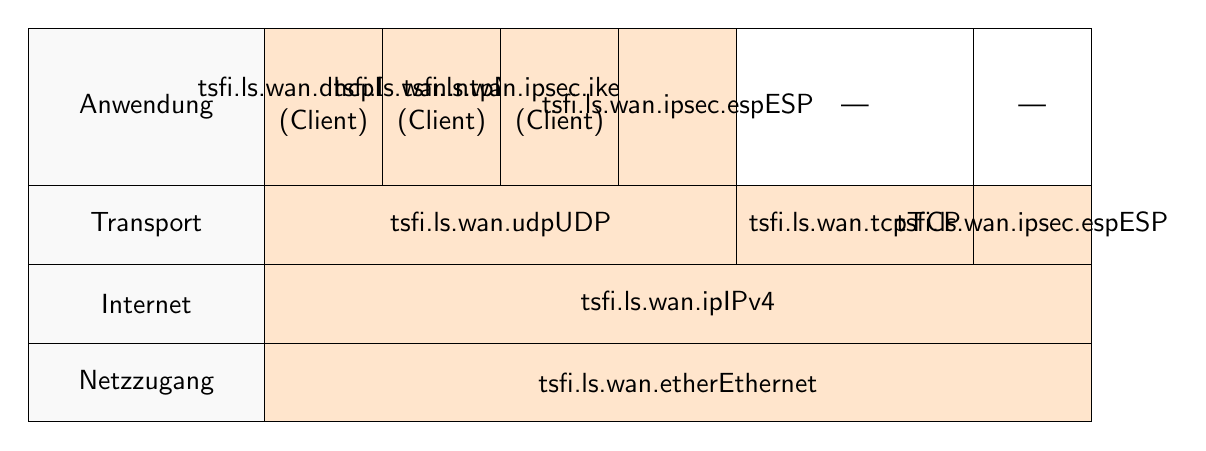
\begin{tikzpicture}
    [c/.style={midway,align=center,font=\sffamily},
      tsfi/.style={fill=orange!20},
      nontsf/.style={fill=yellow!20},
      none/.style={},      
      layer/.style={fill=gray!5}]

  \draw[layer] (0,0) rectangle ++(3,1) node[c]{Netzzugang};
  \draw[tsfi] (3,0) rectangle ++(10.5,1) node[c]{\hyperlink{tsfi.ls.wan.ether}{Ethernet}};

  \draw[layer] (0,1) rectangle ++(3,1) node[c]{Internet};
  \draw[tsfi] (3,1) rectangle ++(10.5,1) node[c]{\hyperlink{tsfi.ls.wan.ip}{IPv4}};

  \draw[layer] (0,2) rectangle ++(3,1) node[c]{Transport};
  \draw[tsfi] (3,2) rectangle ++(6,1) node[c]{\hyperlink{tsfi.ls.wan.udp}{UDP}};
  \draw[tsfi] (9,2) rectangle ++(3,1) node[c]{\hyperlink{tsfi.ls.wan.tcp}{TCP}};
  \draw[tsfi] (12,2) rectangle ++(1.5,1) node[c]{\hyperlink{tsfi.ls.wan.ipsec.esp}{ESP}};

  \draw[layer] (0,3) rectangle ++(3,2) node[c]{Anwendung};
  \draw[tsfi] (3,3) rectangle ++(1.5,2) node[c]{\hyperlink{tsfi.ls.wan.dhcp}{DHCP} \\ (Client)};
  \draw[tsfi] (4.5,3) rectangle ++(1.5,2) node[c]{\hyperlink{tsfi.ls.wan.ntp}{NTP} \\ (Client)};
  \draw[tsfi] (6,3) rectangle ++(1.5,2) node[c]{\hyperlink{tsfi.ls.wan.ipsec.ikev2}{IKEv2} \\ (Client)};
  \draw[tsfi] (7.5,3) rectangle ++(1.5,2) node[c]{\hyperlink{tsfi.ls.wan.ipsec.esp}{ESP}};
  \draw[none] (9,3) rectangle ++(3,2) node[c]{---};
  \draw[none] (12,3) rectangle ++(1.5,2) node[c]{---};

\end{tikzpicture}
  \caption{Protokolle auf \formatintf{LS.WAN} für die sicherheitsfunktionalen Anteile}
  \label{fig:tsfi.ls.wan.protocols}
\end{figure}


\hrefsubsection{tsfi.ls.wan.ether}{\tsfisectionname{ls.wan.ether}}

\sameprotocol{Ethernet}{WAN}{tsfi.ls.lan.ether}

\hrefsubsection{tsfi.ls.wan.ip}{\tsfisectionname{ls.wan.ip}}

\sameprotocol{IPv4 und ICMP}{WAN}{tsfi.ls.lan.ip}

\hrefsubsection{tsfi.ls.wan.tcp}{\tsfisectionname{ls.wan.tcp}}

\sameprotocol{TCP}{WAN}{tsfi.ls.lan.tcp}

\hrefsubsection{tsfi.ls.wan.udp}{\tsfisectionname{ls.wan.udp}}

\sameprotocol{UDP}{WAN}{tsfi.ls.lan.udp}

\hrefsubsection{tsfi.ls.wan.dhcp}{\tsfisectionname{ls.wan.dhcp}}

\tsfipurpose{tsfi.ls.wan.dhcp}

Der TOE bietet die Möglichkeit, auf der WAN-Schnittstelle als
DHCP-Client zu agieren. Der TOE kann also seine IP-Adresse von einem
DHCP-Server im WAN beziehen. Diese Funktion ist auf der Managementoberfläche
(de-)aktivierbar.

\calledsfmanual{ls.wan.dhcp}{\secfunclink{sf.networkservices}}

\tsfiparameters{tsfi.ls.wan.dhcp}

Das DHCP-Protokoll setzt auf dem UDP-Protokoll auf und ist in
\rfc[c]{2131} beschrieben. Die Beschreibungen enthalten
insbesondere das Format einer DHCP-Nachricht und die darin
enthaltenen Felder, die verschiedenen Nachrichtentypen und den Ablauf
der Kommunikation.

Das \rfc[c]{2132} dokumentiert zudem weitere DHCP-Optionen,
die der DHCP-Server mit dem DHCP-Client austauschen kann.

\hrefsubsection{tsfi.ls.wan.ntp}{\tsfisectionname{ls.wan.ntp}}

\tsfipurpose{tsfi.ls.wan.ntp}

Die Schnittstelle wird genutzt, um die Systemzeit mit Zeitservern aus dem
Internet zu synchronisieren. (\sfrlink{fpt_stm.1})

\calledsf{ls.wan.ntp}

\tsfiparameters{tsfi.ls.wan.ntp}

Die Protokollbeschreibung ist in \rfc[c]{5905}
dokumentiert. Der Zielport für den Client ist UDP-Port~123.

\hrefsubsection{tsfi.ls.wan.ipsec}{\tsfisectionname{ls.wan.ipsec}}

\tsfipurpose{tsfi.ls.wan.ipsec}

Der TOE verwendet die WAN-Schnittstelle für den Aufbau des VPN-Kanals Der TOE
bietet dafür IPsec als VPN-Client an der WAN-Schnittstelle an.

\calledsf{ls.wan.ipsec}

\tsfiparameters{tsfi.ls.wan.ipsec}

IPSec berücksichtigt die Vorgaben aus \rfc[c]{4301}. Der TOE verwendet
für IPSec zwei Protokolle. Zum Schlüsselaustausch wird das Protokoll
Internet Key Exchange (IKE) in der Version 2 nach \rfc[c]{7296}
am UDP-Port~500 verwendet. Für die Übertragung der Nutzdaten wird das
Encapsulation Security Payload (ESP) nach \rfc[c]{4303}
(IP-Protokollnummer 50, bzw. UDP-Port 4500) umgesetzt.

\hrefsubsubsection{tsfi.ls.wan.ipsec.ikev2}{Internet Key Exchange Version 2 (IKEv2)}

IKE selbst ist nicht für die Übertragung von Nutzdaten verantwortlich, sondern
lediglich für die Verteilung von geeignetem Schlüsselmaterial und die
Authentifizierung der zwei Parteien. Die Übertragung der eigentlichen Nutzdaten
ist die Aufgabe des ESP-Protokolls
(vgl. Abschnitt~\vref{tsfi.ls.wan.ipsec.esp}).

Der TOE als Initiator der VPN-Verbindungen schlägt zu Beginn des IKE-Protokolls
die zu verwendenden Algorithmen vor.


\hrefsubsubsection{tsfi.ls.wan.ipsec.esp}{Encrypted Security Payload (ESP)}

Das ESP-Protokoll gewährleistet Authentizität, Integrität und
Vertraulichkeit der übermittelten Daten. Dabei werden getrennte
Algorithmen für Verschlüsselung und Integritätssicherung verwendet.

Die in IKE für ESP ausgehandelte SA inklusive der benötigen Schlüssel
und Algorithmen wird nun verwendet, um die IP-Pakete, die über den
Tunnel verschickt werden sollen, zu sichern. Dazu wird die Struktur
des ESP-Headers verwendet, wie in
\figureref{fig:tsfi.ls.wan.ipsec.esp.header} dargestellt
(s.\,a. \cite[Figure~2]{rfc4303})


\begin{figure}[htbp]
  \centering
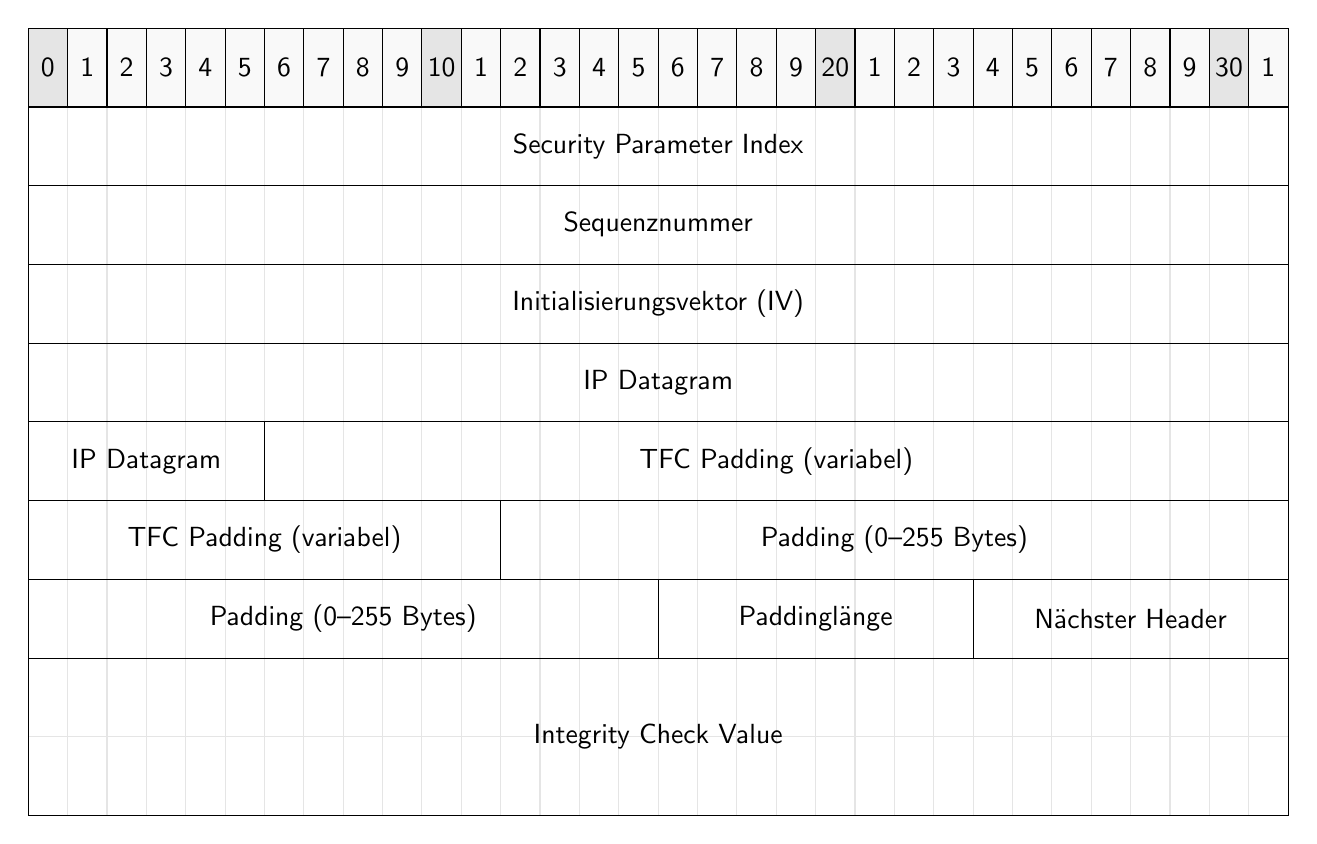
\begin{tikzpicture}
  [c/.style={midway,font=\sffamily},
  none/.style={},
  index/.style={fill=gray!5},
  index0/.style={fill=gray!20}]

  \draw[xstep=.5,gray!20, thin] (0,0) grid (16,9);

  \draw[index] (15.5,9) rectangle ++(0.5,1) node[c]{1};
  \draw[index0] (15,9) rectangle ++(0.5,1) node[c]{30};
  \draw[index] (14.5,9) rectangle ++(0.5,1) node[c]{9};
  \draw[index] (14,9) rectangle ++(0.5,1) node[c]{8};
  \draw[index] (13.5,9) rectangle ++(0.5,1) node[c]{7};
  \draw[index] (13,9) rectangle ++(0.5,1) node[c]{6};
  \draw[index] (12.5,9) rectangle ++(0.5,1) node[c]{5};
  \draw[index] (12,9) rectangle ++(0.5,1) node[c]{4};
  \draw[index] (11.5,9) rectangle ++(0.5,1) node[c]{3};
  \draw[index] (11,9) rectangle ++(0.5,1) node[c]{2};
  \draw[index] (10.5,9) rectangle ++(0.5,1) node[c]{1};
  \draw[index0] (10,9) rectangle ++(0.5,1) node[c]{20};
  \draw[index] (9.5,9) rectangle ++(0.5,1) node[c]{9};
  \draw[index] (9,9) rectangle ++(0.5,1) node[c]{8};
  \draw[index] (8.5,9) rectangle ++(0.5,1) node[c]{7};
  \draw[index] (8,9) rectangle ++(0.5,1) node[c]{6};
  \draw[index] (7.5,9) rectangle ++(0.5,1) node[c]{5};
  \draw[index] (7,9) rectangle ++(0.5,1) node[c]{4};
  \draw[index] (6.5,9) rectangle ++(0.5,1) node[c]{3};
  \draw[index] (6,9) rectangle ++(0.5,1) node[c]{2};
  \draw[index] (5.5,9) rectangle ++(0.5,1) node[c]{1};
  \draw[index0] (5,9) rectangle ++(0.5,1) node[c]{10};
  \draw[index] (4.5,9) rectangle ++(0.5,1) node[c]{9};
  \draw[index] (4,9) rectangle ++(0.5,1) node[c]{8};
  \draw[index] (3.5,9) rectangle ++(0.5,1) node[c]{7};
  \draw[index] (3,9) rectangle ++(0.5,1) node[c]{6};
  \draw[index] (2.5,9) rectangle ++(0.5,1) node[c]{5};
  \draw[index] (2,9) rectangle ++(0.5,1) node[c]{4};
  \draw[index] (1.5,9) rectangle ++(0.5,1) node[c]{3};
  \draw[index] (1,9) rectangle ++(0.5,1) node[c]{2};
  \draw[index] (0.5,9) rectangle ++(0.5,1) node[c]{1};
  \draw[index0] (0,9) rectangle ++(0.5,1) node[c]{0};

  \draw[none] (0,8) rectangle ++(16,1) node[c]{Security Parameter Index};

  \draw[none] (0,7) rectangle ++(16,1) node[c]{Sequenznummer};

  \draw[none] (0,6) rectangle ++(16,1) node[c]{Initialisierungsvektor (IV)};

  \draw[none] (0,5) rectangle ++(16,1) node[c]{IP Datagram};

  \draw[none] (3,4) rectangle ++(13,1) node[c]{TFC Padding (variabel)};
  \draw[none] (0,4) rectangle ++(3,1) node[c]{IP Datagram};

  \draw[none] (6,3) rectangle ++(10,1) node[c]{Padding~(0--255 Bytes)};
  \draw[none] (0,3) rectangle ++(6,1) node[c]{TFC Padding (variabel)};

  \draw[none] (12,2) rectangle ++(4,1) node[c]{Nächster Header};
  \draw[none] (8,2) rectangle ++(4,1) node[c]{Paddinglänge};
  \draw[none] (0,2) rectangle ++(8,1) node[c]{Padding~(0--255 Bytes)};

  \draw[none] (0,0) rectangle ++(16,2) node[c]{Integrity Check Value};

\end{tikzpicture}
  \caption{ESP Header}
  \label{fig:tsfi.ls.wan.ipsec.esp.header}
\end{figure}



% !TEX root = "../adv_fsp"
%%% Local Variables:
%%% mode: latex
%%% TeX-engine: luatex
%%% TeX-master: "../adv_fsp"
%%% TeX-parse-self: t
%%% TeX-auto-save: t
%%% End:


\clearpage


\hrefsection{tsfi.ls.led}{\tsfisectionname{ls.led}}

Über diese Schnittstelle kann der TOE des Status auf \intf{PS.LED}
anzeigen. \lsled{} wird vom Betriebssystem genutzt. Die Bedeutung der Anzeige
ist in \autocite[Kapitel 6]{agd_adm} beschrieben.


% !TEX root = adv_fsp
%%% Local Variables:
%%% mode: latex
%%% TeX-engine: luatex
%%% TeX-master: "adv_fsp"
%%% TeX-parse-self: t
%%% TeX-auto-save: t
%%% End:
